% Chapter 5: Project Documentation
\chapter{Project Documentation}

\section{Implementation}
The implementation of this system involves integrating key components: \textbf{image capture}, \textbf{face detection}, \textbf{face classification}, and \textbf{attendance logging}. Each component contributes to the system's capability to perform real-time, accurate face recognition.

\begin{itemize}
    \item \textbf{Image Capture}: The system initiates by capturing images through a connected camera. This module is designed to automatically capture facial images when individuals are within a defined range.
    
    \item \textbf{Face Detection}: Using the \textbf{OpenCV} library, the system detects face locations within the captured images. This step is optimized for quick, precise detection, even under varied lighting conditions.
    
    \item \textbf{Face Recognition with YOLOv8m}: The \textbf{YOLOv8m} model, trained on a specialized dataset, classifies detected faces accurately. The model is implemented using \textbf{TensorFlow}, allowing fast inference within the application.
    
    \item \textbf{Attendance Logging}: Recognized faces are logged in the attendance module, with each entry stored in a database, capturing time and identity details. This module can also generate reports for daily or monthly attendance monitoring.
\end{itemize}

\section{Results and Discussion}

\subsection{Model Training and Evaluation}
\begin{itemize}
    \item \textbf{Dataset and Annotation}: The dataset used for training contains 3,873 face images across six classes (Ajul, Izzata, Joy, Kelvin, Lia, and Trisman). The \textbf{YOLOv8m} model was selected for its proficiency in diverse detection scenarios.

    \item \textbf{Training Process}: The YOLOv8m model was trained using the \textbf{AdamW} optimizer with a learning rate of \textbf{0.001} and momentum of \textbf{0.9} over \textbf{100 epochs}. Data augmentations such as blurring and grayscale conversion improved robustness. A validation set of \textbf{774 images} ensured generalization.
\end{itemize}

\begin{figure}[htbp]
    \centering
    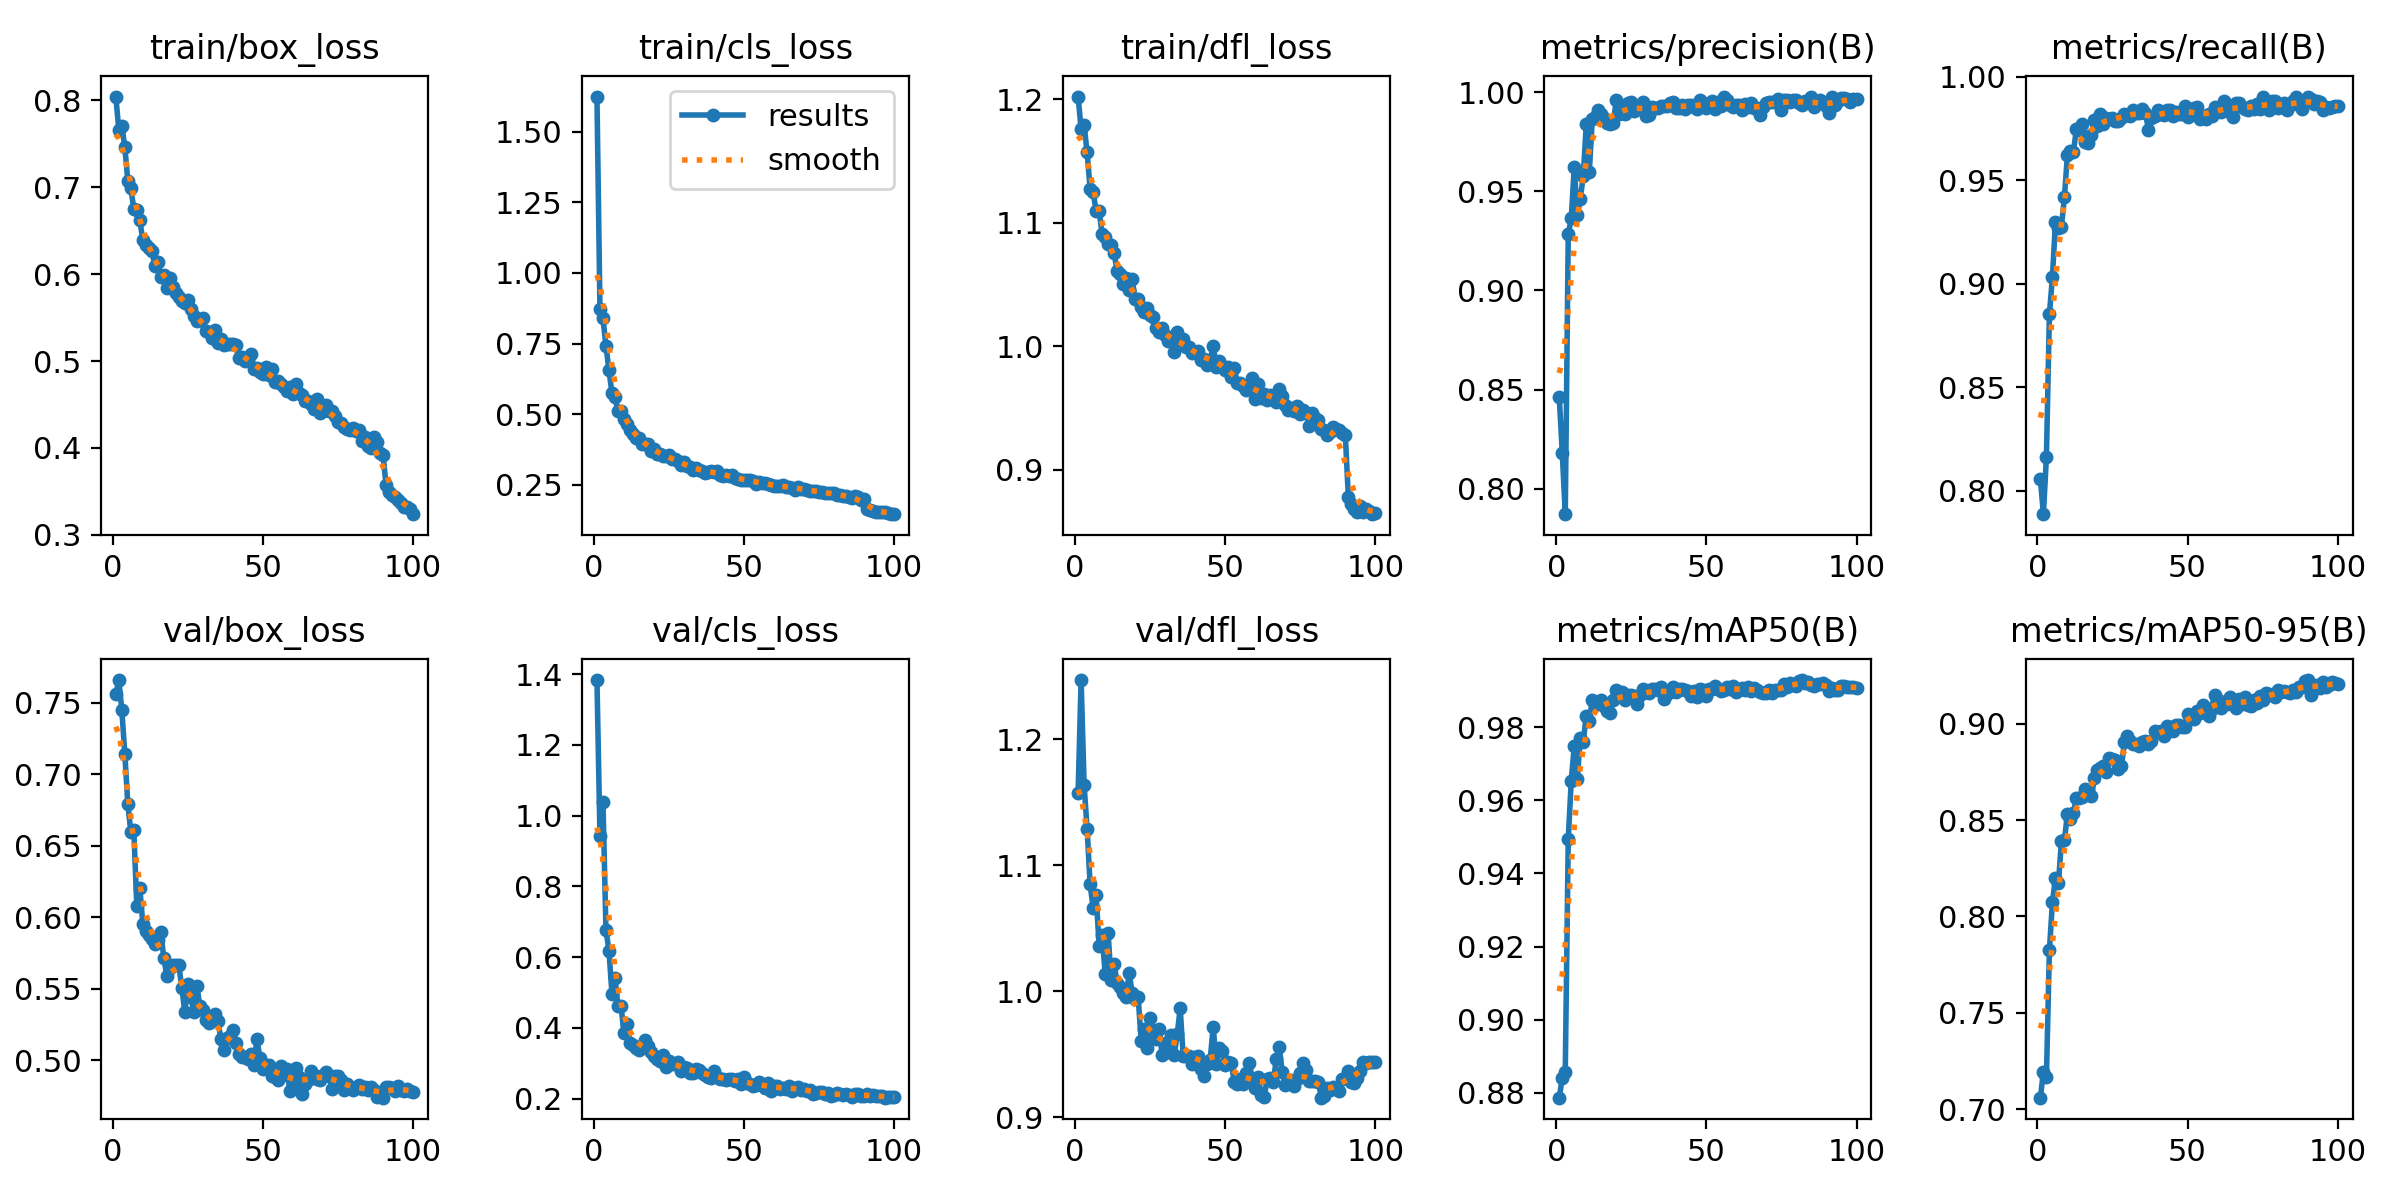
\includegraphics[width=0.8\textwidth]{images/results.png}
    \caption{Training Results of YOLOv8m Model}
    \label{fig:training_results}
\end{figure}

\subsection{Precision-Recall Analysis}
The \textbf{Precision-Recall curve} yielded an average precision of \textbf{0.995} across all classes, indicating strong class distinction. Each class (Ajul, Izzata, Joy, Kelvin, Lia, and Trisman) scored a precision of \textbf{0.995} at high recall, demonstrating effective classification with minimal errors.

\begin{figure}[htbp]
    \centering
    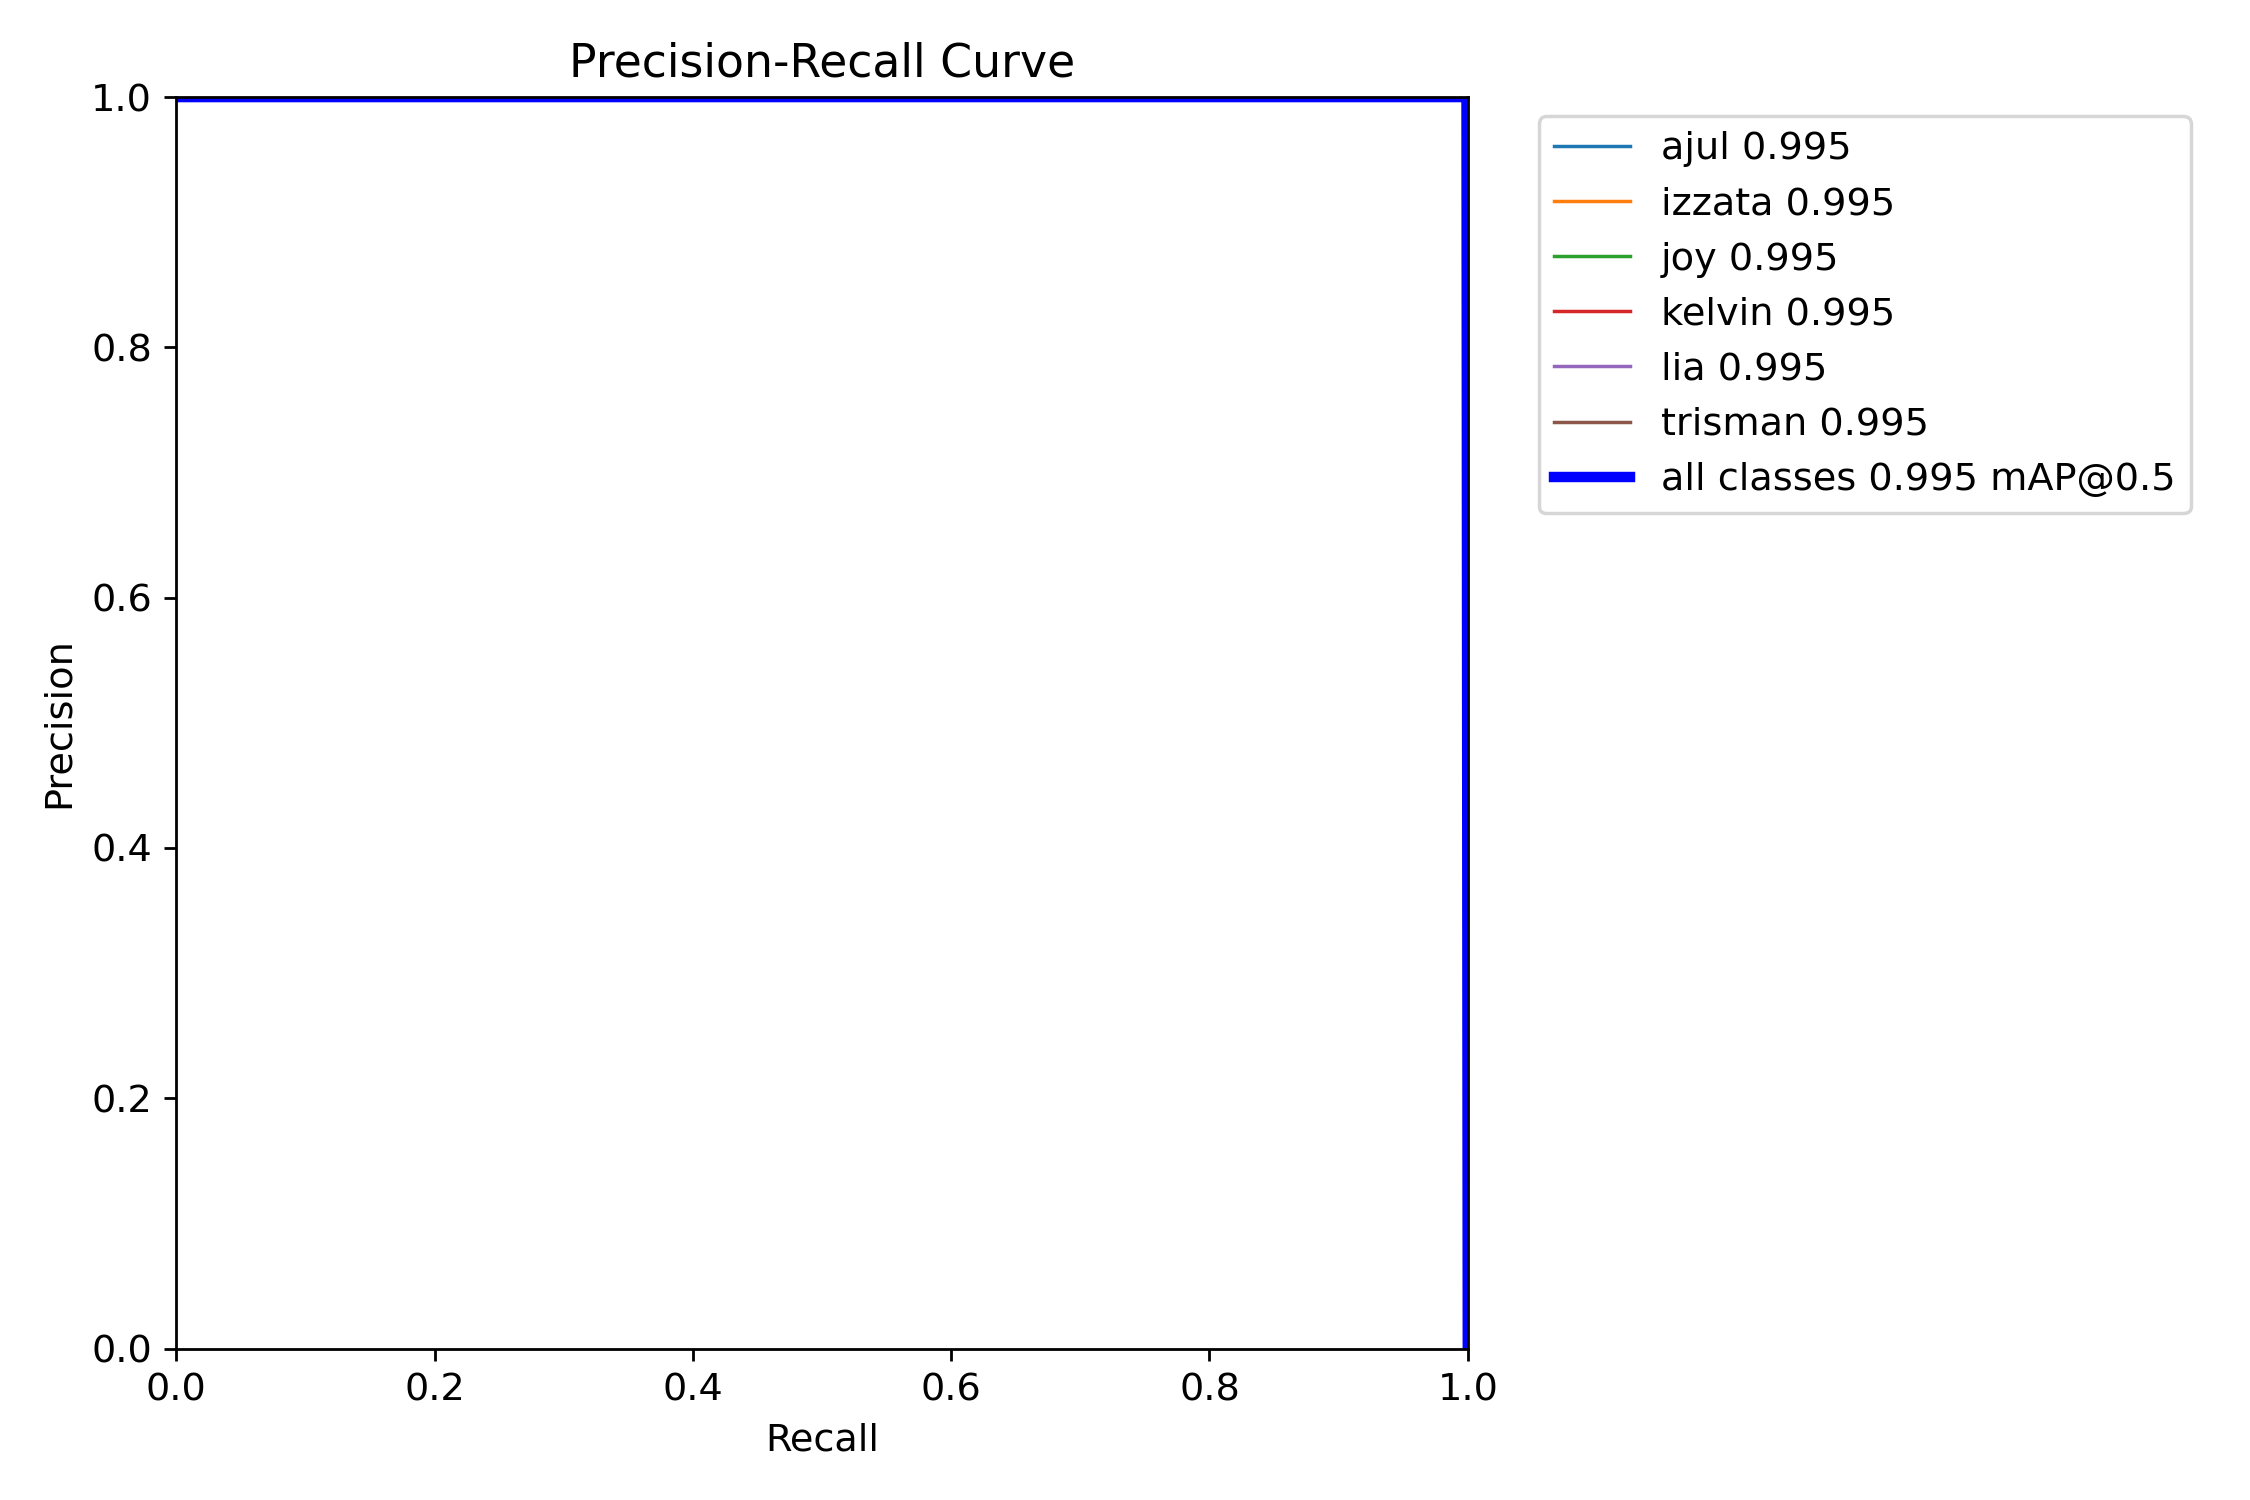
\includegraphics[width=0.8\textwidth]{images/PR_curve (1).png}
    \caption{Precision-Recall Curve for YOLOv8m Model}
    \label{fig:pr_curve}
\end{figure}

\subsection{F1-Confidence Analysis}
The \textbf{F1-Confidence curve} shows an F1 score of \textbf{1.00} for all classes at a confidence level of \textbf{0.8}. This suggests the model’s high precision and accuracy. The F1 score remains stable at higher confidence levels, reinforcing its reliability in face classification.

\begin{figure}[htbp]
    \centering
    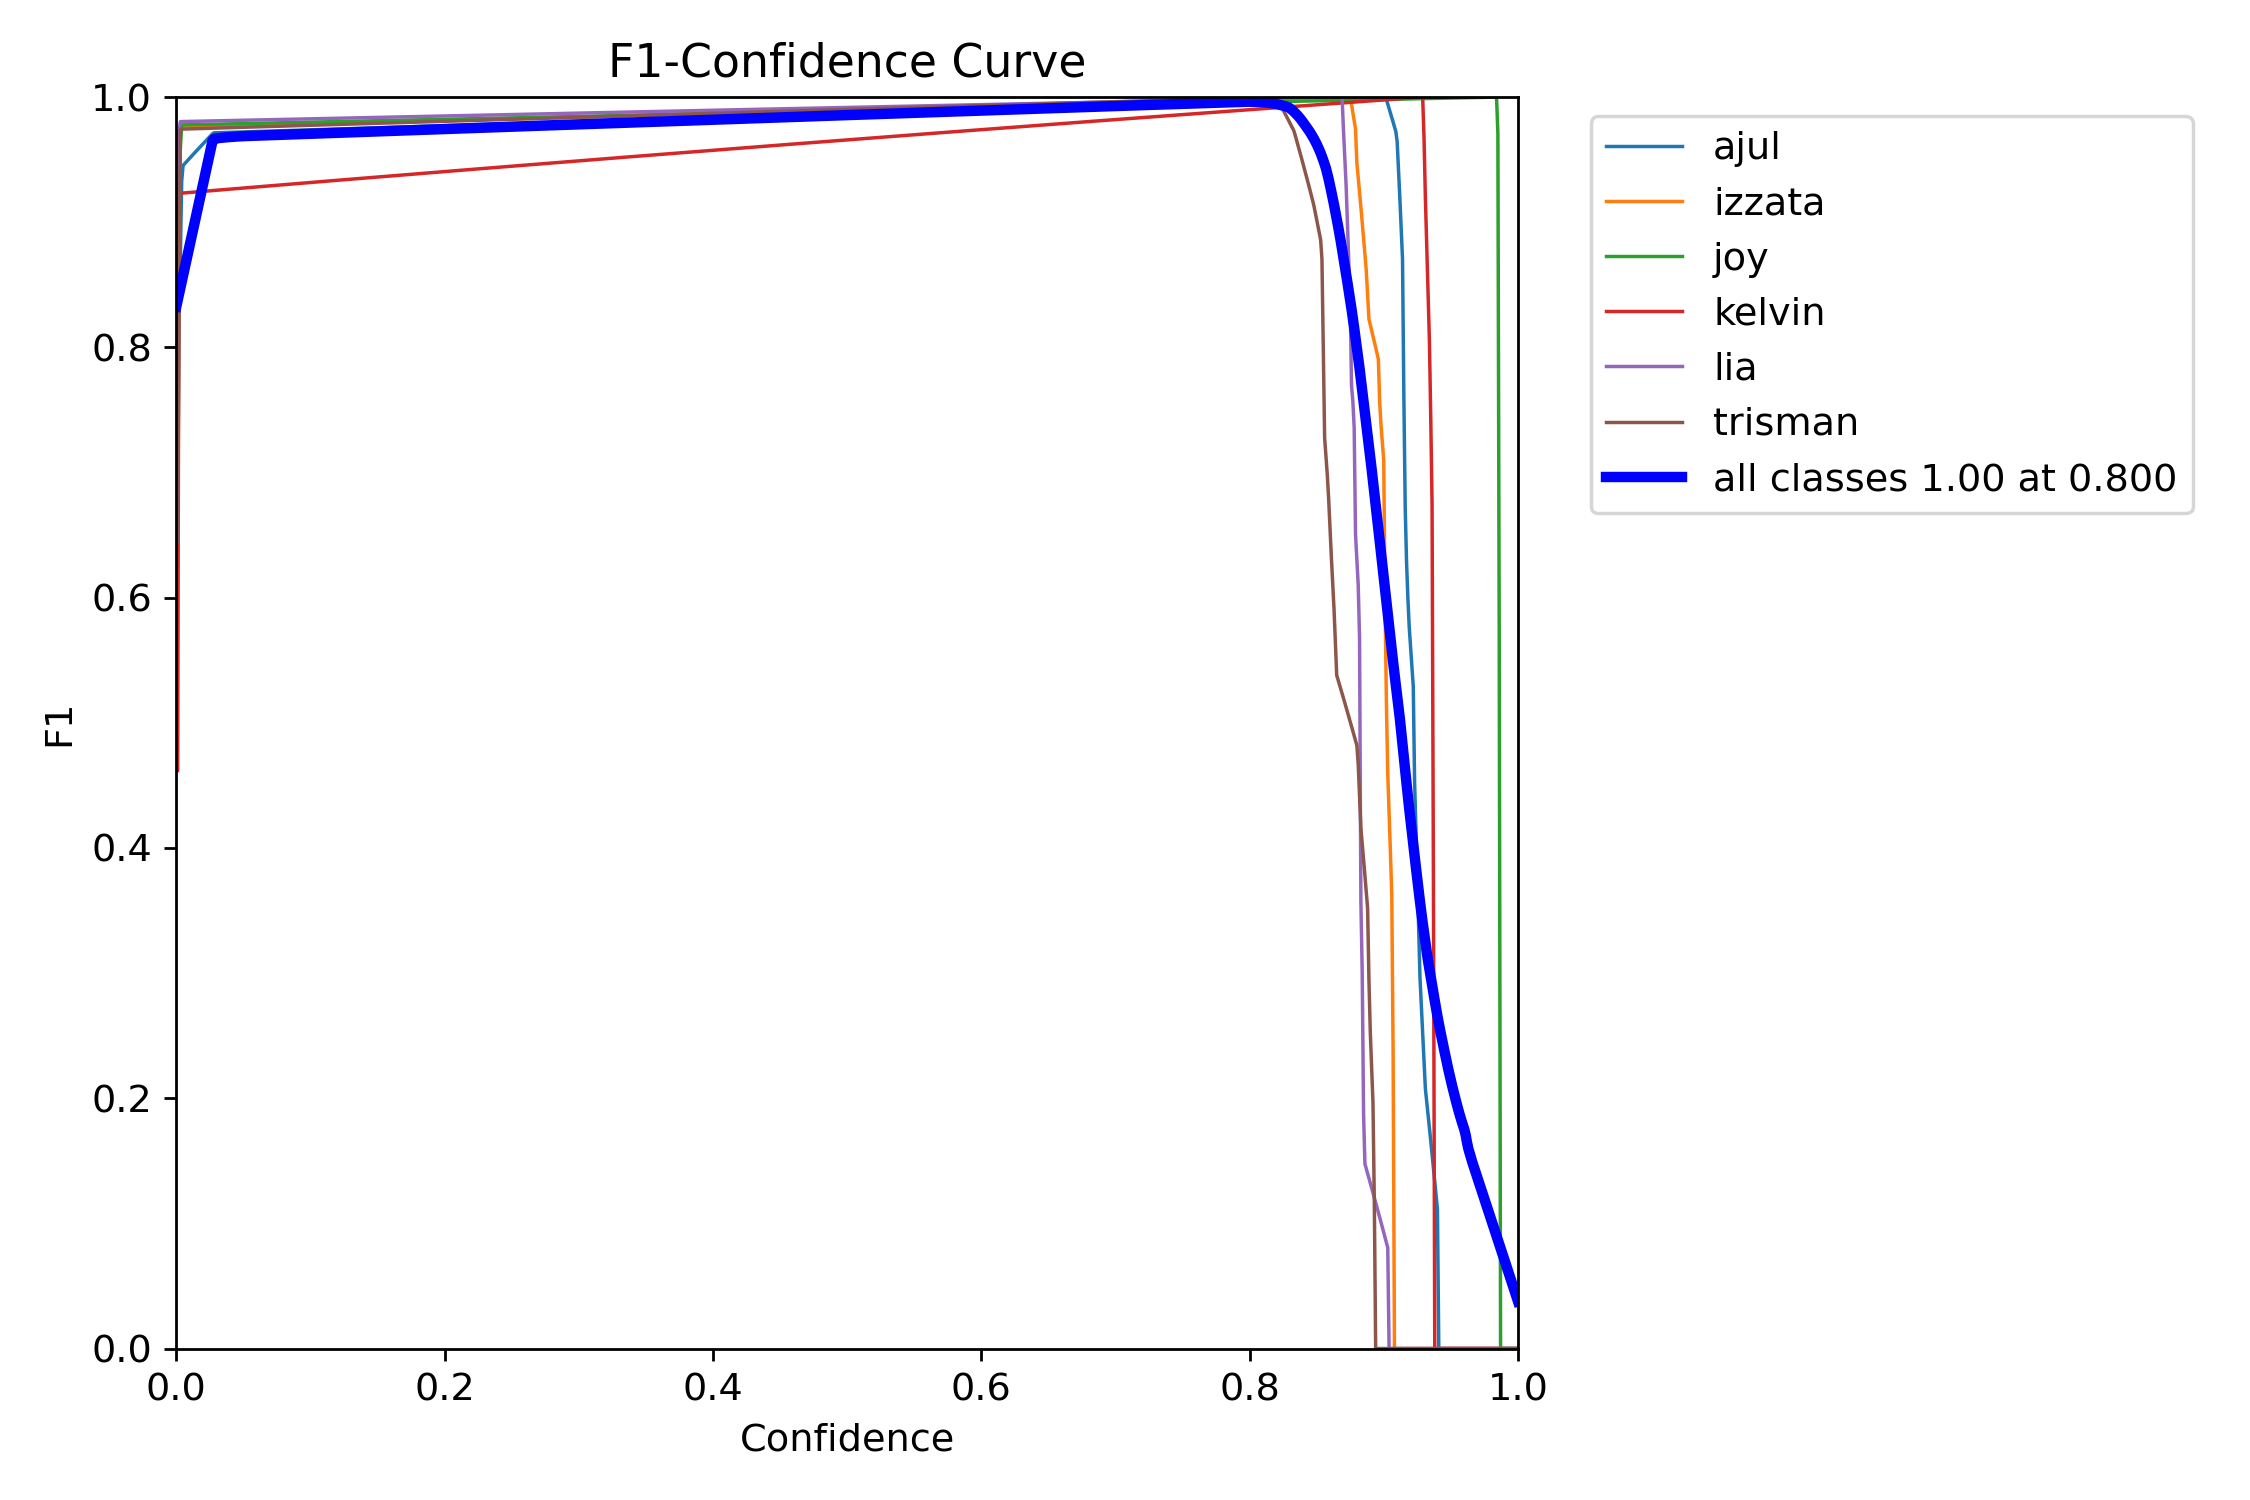
\includegraphics[width=0.8\textwidth]{images/F1_curve.png}
    \caption{F1-Confidence Curve for YOLOv8m Model}
    \label{fig:f1_curve}
\end{figure}

\subsection{Performance Summary}
The model achieved a mean Average Precision (mAP@0.5) of \textbf{0.995}, demonstrating strong performance in face recognition. This level of accuracy positions the model as suitable for applications demanding high precision, such as attendance systems or security monitoring.

\section{Conclusion}
The YOLOv8m model’s high precision, recall, and F1 scores across all classes indicate its effectiveness in recognizing and differentiating between individuals with minimal misclassification. The model’s performance confirms its viability for deployment in real-world applications that require accurate and reliable face recognition.
